%%%%%%%%%%%%%%%%%%%%%%%%%%%%%%%%%%%%
%% Template file SP 2024
%% Include in directory homework.sty and headerfooter.tex
%%%%%%%%%%%%%%%%%%%%%%%%%%%%%%%%%%%%

\documentclass[12pt]{article}
\usepackage{homework}

\graphicspath{{images/}}
\geometry{letterpaper, portrait, includeheadfoot=true, hmargin=1in, vmargin=1in}

\setcounter{section}{-1}
%% Solution hiding %%
\usepackage[utf8]{inputenc}
\usepackage{lipsum}


\begin{document}
\singlespacing

\renewcommand{\familydefault}{\rmdefault}
\pagestyle{fancy}
\fancyhf{}
\setlength{\headheight}{30pt}
\renewcommand{\headrulewidth}{0.4pt}
\renewcommand{\footrulewidth}{0.4pt}
\lhead{\large Homework 2 \\ Due Feb. 20, 2024 }
\rhead{\large CS 446 \\ Spring 2024}
\rfoot{\textbf{Page \thepage}}
\lfoot{}

\section{Instructions}

Homework is due Tuesday, March 18, 2024 at 23:59pm Central Time.
Please refer to \url{https://courses.grainger.illinois.edu/cs446/sp2024/homework/hw/index.html} for course policy on homeworks and submission instructions.

\section{Neural networks for simple functions}
\begin{enumerate}
    \item   \[w_0 = w_1 = [1, -1]^{\top}\]
    \item   \[w_0 = [1, -1]^{\top}, \, w_1 = [m, -m]^{\top}, \, b = [\frac{b}{m}, -\frac{b}{m}]^{\top}\]
    \item   \[w_0 = 0, \, w_1 = 2b\]
    \item   \[w_0 = [1, 1, 1]^{\top}, \, b_0 = [2, 0,-2]^{\top}, \, w_1 = [3, -6, 3]^{\top}\]
    \item   No. $x^2 = |x|^2$, while any transformation in $f(x)$ is either making linear transforms ($w$), or resulting in 0 ($\sigma$), in which $0 \leq |x|$. Any combination of them is impossible to produce a quadratic transform.
    \item   No. For $w_0x + b_0 > 0$, $|f(x) - x^2| = |w_1^{\top}w_0x - x^2 + w_1^{\top}b_0|$. For $w_0x + b_0 \leq 0$, $|f(x) - x^2| = |0 - x^2|$. Both of them are quadratic functions on $x$ that will explode as $x$ grows larger.
    \item   Yes. As $x$ is limited in this case, we can select appropriate parameters to approximate $x^2$ with gradient descent:
    \[\frac{\partial f}{\partial w_1} = \sigma(w_0x + b_0)\]
    \[\frac{\partial f}{\partial w_0} = w_1\cdot\mathds{1}\{x>0\}\cdot x;\; \frac{\partial f}{\partial b_0} = w_1\cdot\mathds{1}\{x>0\}\]
\end{enumerate}
\newpage

\section{Backpropagation through time (BPTT)}
\begin{enumerate}
    \item As below:
    \begin{figure}[htbp]
        \centering
        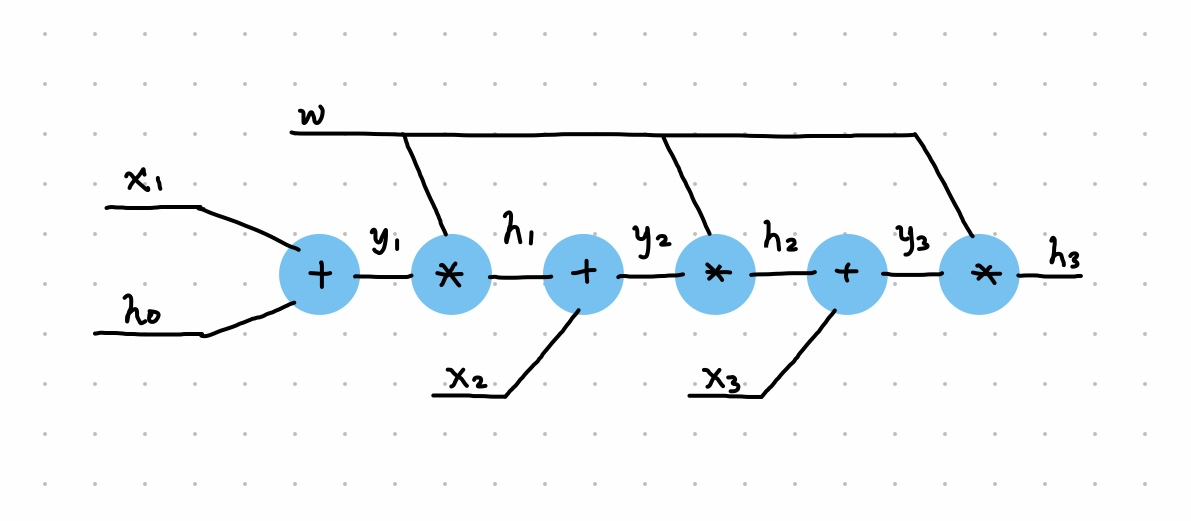
\includegraphics[width=0.6\textwidth]{2.1}
    \end{figure}
    \item   \[h_0 = 0, \, h_1 = w(x_1 + h_0) = wx_1, \, h_2 = w(x_2 + h_1) = wx_2 + w^2x_1,\] 
    \[h_3 = w(x_3 + h_2) = wx_3 + w^2x_2 + w^3x_1\]
    \[y_1 = x_1 + h_0 = x_1, \, y_2 = x_2 + h_1 = x_2 + wx_1, \, y_3 = x_3 + h_2 = x_3 + wx_2 + w^2x_1\]
    \item   \[\frac{\partial h_3}{\partial w} = x_3 + (h_2 + w\frac{\partial h_2}{\partial w}) = x_3 + wx_2 + w^2x_1 + w[x_2 + (h_1 + w\frac{\partial h_1}{\partial w})]\] 
    \[= x_3 + 2wx_2 + 2w^2x_1 + w^2(\frac{\partial h_1}{\partial w}) = x_3 + 2wx_2 + 3w^2x_1\]
    \item   \[\frac{\partial f}{\partial h_1} = \frac{\partial h_T}{\partial h_1} = \prod_{t = 1}^{T-1} \frac{\partial h_{t+1}}{\partial h_t} = \prod_{t = 1}^{T-1} w\sigma'(x_t + h_{t-1}) = w^{T-1}\prod_{t = 1}^{T-1} \sigma'(x_t + h_{t-1})\]
    \item   From the previous question we can see that if $w$ is initialized too large or gradient components are mostly larger than 1 during the propagation, the gradient will tend to explode. In other cases that $w$ is initialized small or gradient components are mostly less than 1, the gradient will tend to diminish to 0.
\end{enumerate}
\newpage

\section{Transformers}
\begin{enumerate}
    \item Theoretically $\alpha_i$ can't be infinitely large since attention weights are supposed to be designed between 0 and 1. Practically the numerator in $\alpha_i$ would be less than denominator, and both of them can't reach 0 due to exponential. In this way, $\alpha_i$ can neither be neither infinitely large nor be 0.
    \item $q$ and $k_i$ are pointing to similar directions, which differs from the rest $k$. $c = \sum \alpha_i v_i$ for all $i$ satisfying such condition. This means that the token corresponding to $q$ here is attached with greater attention to tokens corresponding to such $i$.
    \item $q = m(k_1 + k_2)$, in which $m$ is a really large number. In this case, we $\exp(k_i^{\top}q) = 1$ for $i\neq 1, 2$ and $\exp(k_i^{\top}q) = \exp(m)$ for $i \in \{1, 2\}$. If $\exp(m) \gg 1$, we have $c \approx \frac{1}{2}(v_1 + v_2)$.
    \item \[\|q - k_i\|_2^2 = \|q\|^2_2 + \|k_i\|^2_2 + 2q^{\top}k_i = \|q\|^2_2 + 2q^{\top}k_i\]
    \[\exp(\frac{-\|q - k_i\|^2_2}{2\sigma}) = \exp(\frac{\|q\|^2_2}{2})\cdot\exp(q^{\top}k_i)\]
    \[\Longrightarrow \beta_i = \frac{\exp(\frac{\|q\|^2_2}{2})\cdot\exp(q^{\top}k_i)}{\exp(\frac{\|q\|^2_2}{2})\cdot\sum_j\exp(q^{\top}k_i)} = \alpha_i\]
    \item Knowing the SVD of $P$, we write $P$ as:
    \[P = U\Sigma V^{\top}\]
    Given $\text{rank}(P) = k$, we have:
    \[P = \sum_{i=1}^k\sigma_i u_i v_i^{\top}\]
    with singular values $\sigma_i$ and singular vectors $u_i, v_i$. There are $n$ of $u_i, v_i$ in dimension $d$, so computation of single $u_i v_i^{\top}$ costs $O(nd)$. Therefore, computation of $P$ above can cost only $O(nkd)$.
\end{enumerate}

\section{Resnet}
\begin{enumerate}
    \item[2.] BatchNorm2d layer will center the output of Conv2d layer around 0, which eliminates the bias.
\end{enumerate}
\newpage

\section{Coding: Image overfitting}
\begin{enumerate}
    \item[5.]
    ReLU:
    \begin{enumerate}
        \item epochs = 500
        \item learning rate = $10^{-4}$
        \item batch size = 800
    \end{enumerate}
    \begin{figure}[ht]
        \centering
        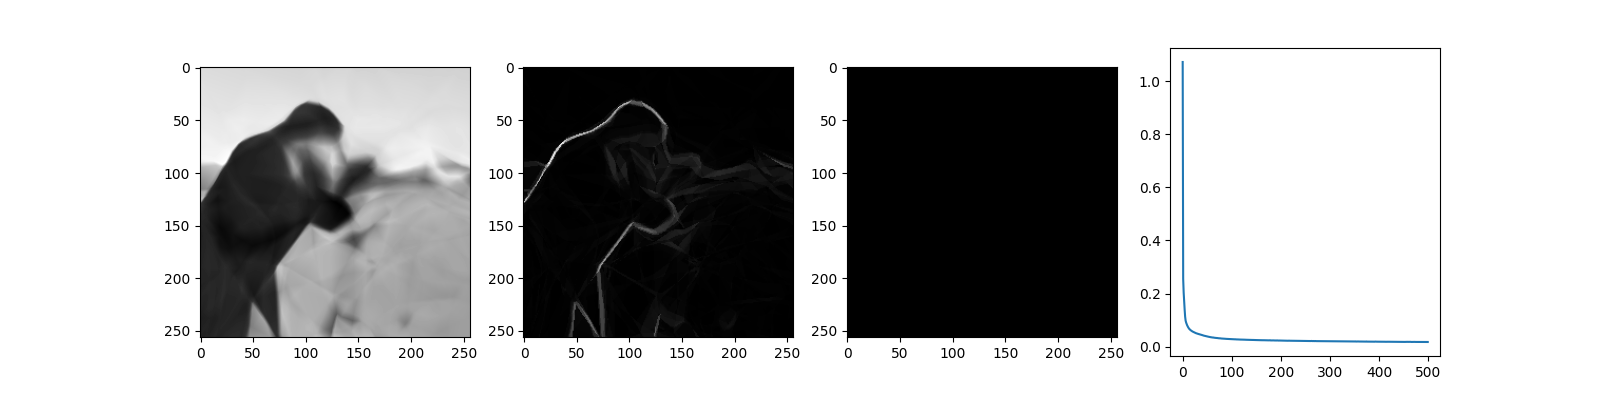
\includegraphics[width=\linewidth]{relu}
    \end{figure}
    Tanh:
    \begin{enumerate}
        \item epochs = 500
        \item learning rate = $10^{-4}$
        \item batch size = 800
    \end{enumerate}
    \begin{figure}[ht]
        \centering
        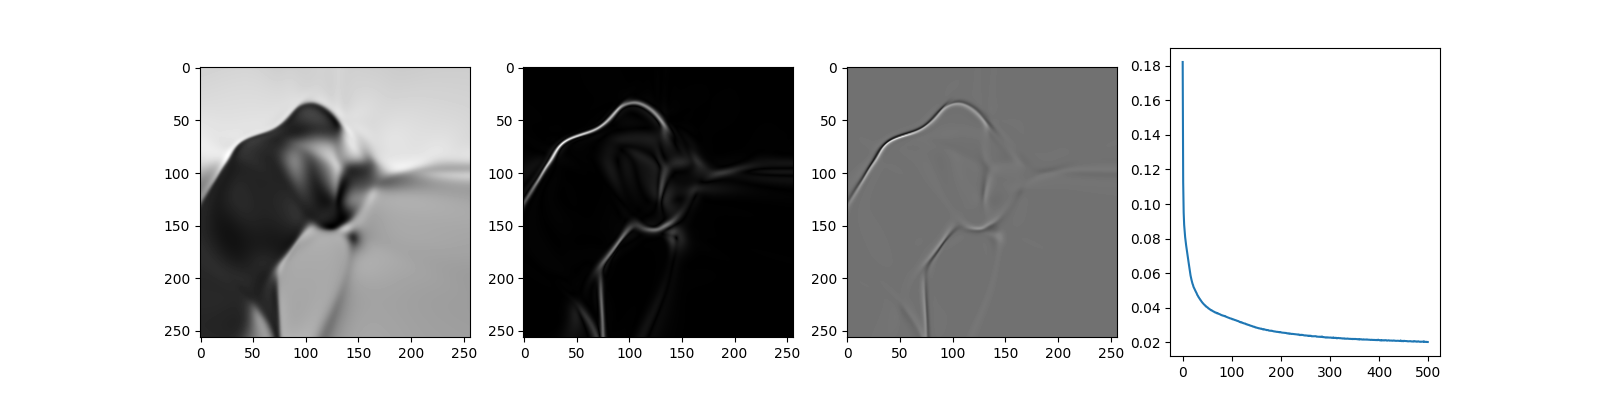
\includegraphics[width=\linewidth]{tanh}
    \end{figure}
    \newpage
    Sin:
    \begin{enumerate}
        \item epochs = 40
        \item learning rate = $10^{-4}$
        \item batch size = 800
    \end{enumerate}
    \begin{figure}[ht]
        \centering
        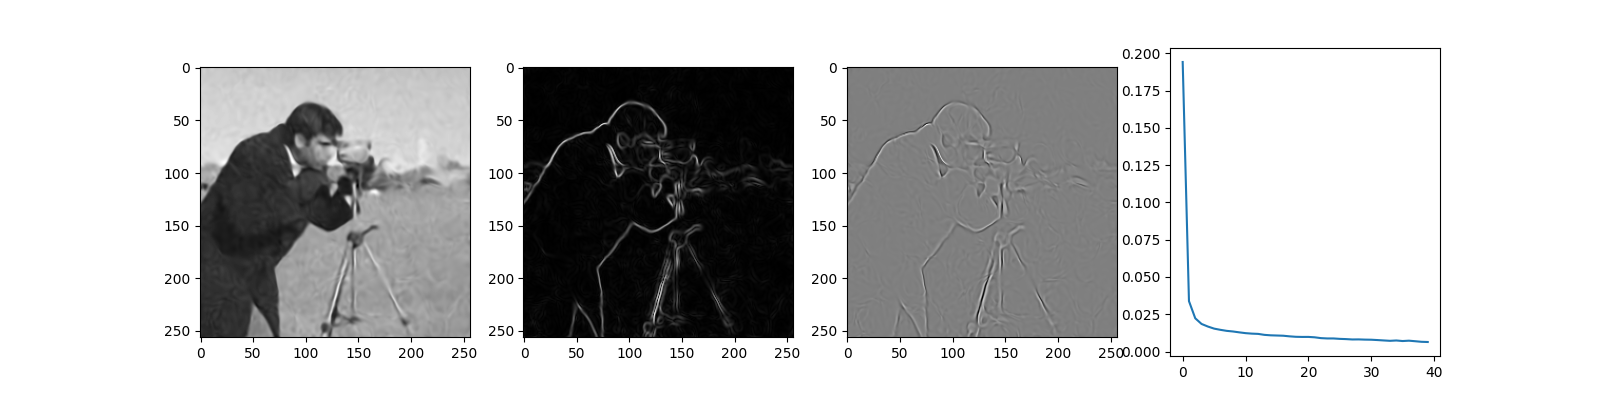
\includegraphics[width=\linewidth]{sin}
    \end{figure}

    \item[6.] \[\nabla^2 \text{ReLU}(\textbf{x}) = \nabla^2 \max\{0, \textbf{x}\} = \frac{\partial^2 \max\{0, \textbf{x}\}}{\partial x_1^2} + \frac{\partial^2 \max\{0, \textbf{x}\}}{\partial x_2^2}\]
    \[= \frac{\partial \mathds{1}\{x>0\}}{\partial x_1} + \frac{\partial \mathds{1}\{x>0\}}{\partial x_2} = 0\]
    \item[7.] Decrease the learning rate appropriately; learning rate scheduling.
    \item[8.] Initial loss is larger, the model converges slower, and the steady loss is higher. The experiment seems failed. Sin activation is picked for the experiment below.
    \begin{enumerate}
        \item epochs = 100
        \item learning rate = $10^{-4}$
        \item batch size = 800
    \end{enumerate}
    \begin{figure}[ht]
        \centering
        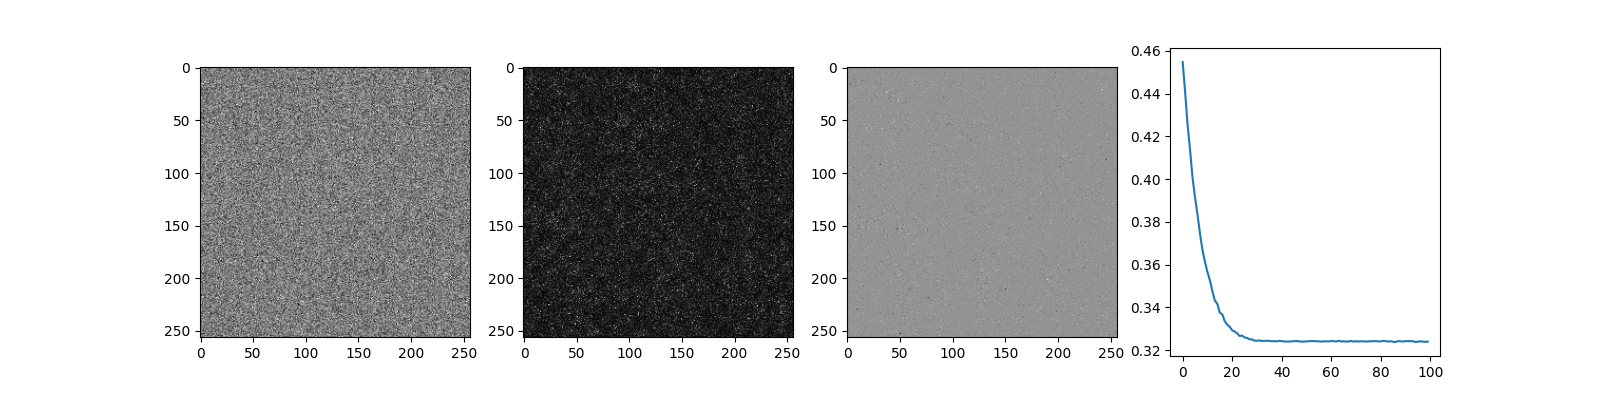
\includegraphics[width=\linewidth]{sin_unini}
    \end{figure}
        
\end{enumerate}
% Resnet code should be submitted on gradescope
% Include plots and results from Q5.5 and written responses for 5.6-8

\end{document}